\newpage
\section{Apprendimento per rinforzo}

L'apprendimento che deriva dall'\textbf{interazione} con un ambiente è una
forma di intelligenza molto comune, la più nota, semplice e intuitiva.

\begin{figure}[H]
\caption{Scenario descrittivo dell'apprendimento per rinforzo}
\centering
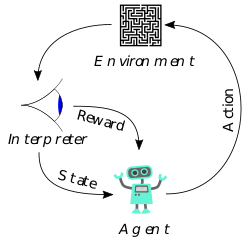
\includegraphics[width=0.5\textwidth]{learning}
\end{figure}

L'apprendimento per rinforzo è guidato da un \textbf{obiettivo}, che viene
usato per stabilire se un'interazione con l'ambiente è positiva o negativa.

L'apprendimento per rinforzo consiste nel sapere quale azione intraprendere in
una data situazione, così da massimizzare la \textbf{ricompensa} (di solito
espressa in forma numerica).

Chi apprende attraverso questo meccanismo deve scoprire quali azioni producono
la maggior ricompensa provandole.

La ricerca ``prova, sbaglia, impara'' e la ``ricompensa con slack'' sono due
importanti concetti.\\

Un agente che apprende deve saper riconoscere lo stato dell'ambiente in cui si trova
e interagire con esso in modo tale da cambiarlo. Deve anche sapere qual è
l'obiettivo da raggiungere.

L'apprendimento per rinforzo è diverso sia dall'apprendimento supervisionato (non
dispone di esempi passati che possano dirgli quale sia la cosa giusta da fare, deve
essere in grado di apprendere da se stesso) che dall'apprendimento non supervisionato
(non deve tentare di trovare patterns o strutture in dati sconosciuti) quello che
deve fare, principalmente, è tentare di massimizzare la ricompensa.

Un agente che apprende deve \textbf{sfruttare} ciò che ha imparato in passato per
ottenere una ricompensa, ma deve anche \textbf{esplorare} nuove azioni per sceglierne
di migliori in futuro.

Questo tipo di approccio permette di gestire le \textbf{incertezze} dell'ambiente in
cui l'agente si trova.

L'effetto di un'azione dell'agente spesso è difficile da prevedere, perciò è necessario
monitorare frequentemente l'ambiente.

(Parentesi psicologica) - tutto ciò si può ricondurre al \textbf{comportamentismo}
(o psicologia comportamentale), un tipo di approccio alla psicologia sviluppato da
John Watson agli inizi del Novecento, basato sull'assunto che il comportamento
esplicito dell'individuo è l'unica unità di analisi scientificamente studiabile della
psicologia avvalendosi del metodo stimolo (ambiente) e risposta (comportamento), in
quanto direttamente osservabile dallo studioso.

\subsection{Elementi del reinforcement learning}

\begin{itemize}
 \item Una \textbf{politica} (mappatura da uno stato dell'ambiente a un'azione da compiere
quando ci si trova in quello stato). Si tratta del cuore di un agente che apprende,
dato che da sola basta per determinarne il comportamento.
 \item Un \textbf{segnale di ricompensa}. Definisce l'obiettivo del problema; a ogni passo
l'agente riceve una ricompensa che deve massimizzare nel lungo termine.
 \item Una \textbf{funzione dei valori}. Mentre la ricompensa definisce ciò che è buono
nel \textbf{breve termine}, la funzione dei valori definisce ciò che è buono nel
\textbf{lungo termine}.
Ne segue che è essenziale prenderla in considerazione quando si devono prendere decisioni/
fare delle valutazioni. Purtroppo i valori sono più difficili da individuare rispetto alla
ricompensa (che è data da uno stimolo dell'ambiente). Di solito occorre osservare tutta
la storia passata di un agente (se disponibile).
Per questo motivo il più importante elemento di un sistema di apprendimento per rinforzo
è proprio quello che effettua la stima dei valori.
 \item Un \textbf{modello dell'ambiente} (opzionale, visto che può essere completamente
ignoto). Viene usato per fare predizioni sui prossimi stati e ricompense se si effettua una
determinata azione. Tale approccio di pianificazione è considerato opposto alla ricerca
``prova, sbaglia, impara''.
\end{itemize}
